\documentclass[tikz, border=10pt]{standalone}

\usepackage{tikz}

\tikzset{
    dot/.style = {fill, circle, inner sep=3pt},
    dashed line/.style = {dash pattern=on3pt off1pt, shorten >=-1.5cm, shorten <=-1.5cm}
}

\begin{document}
    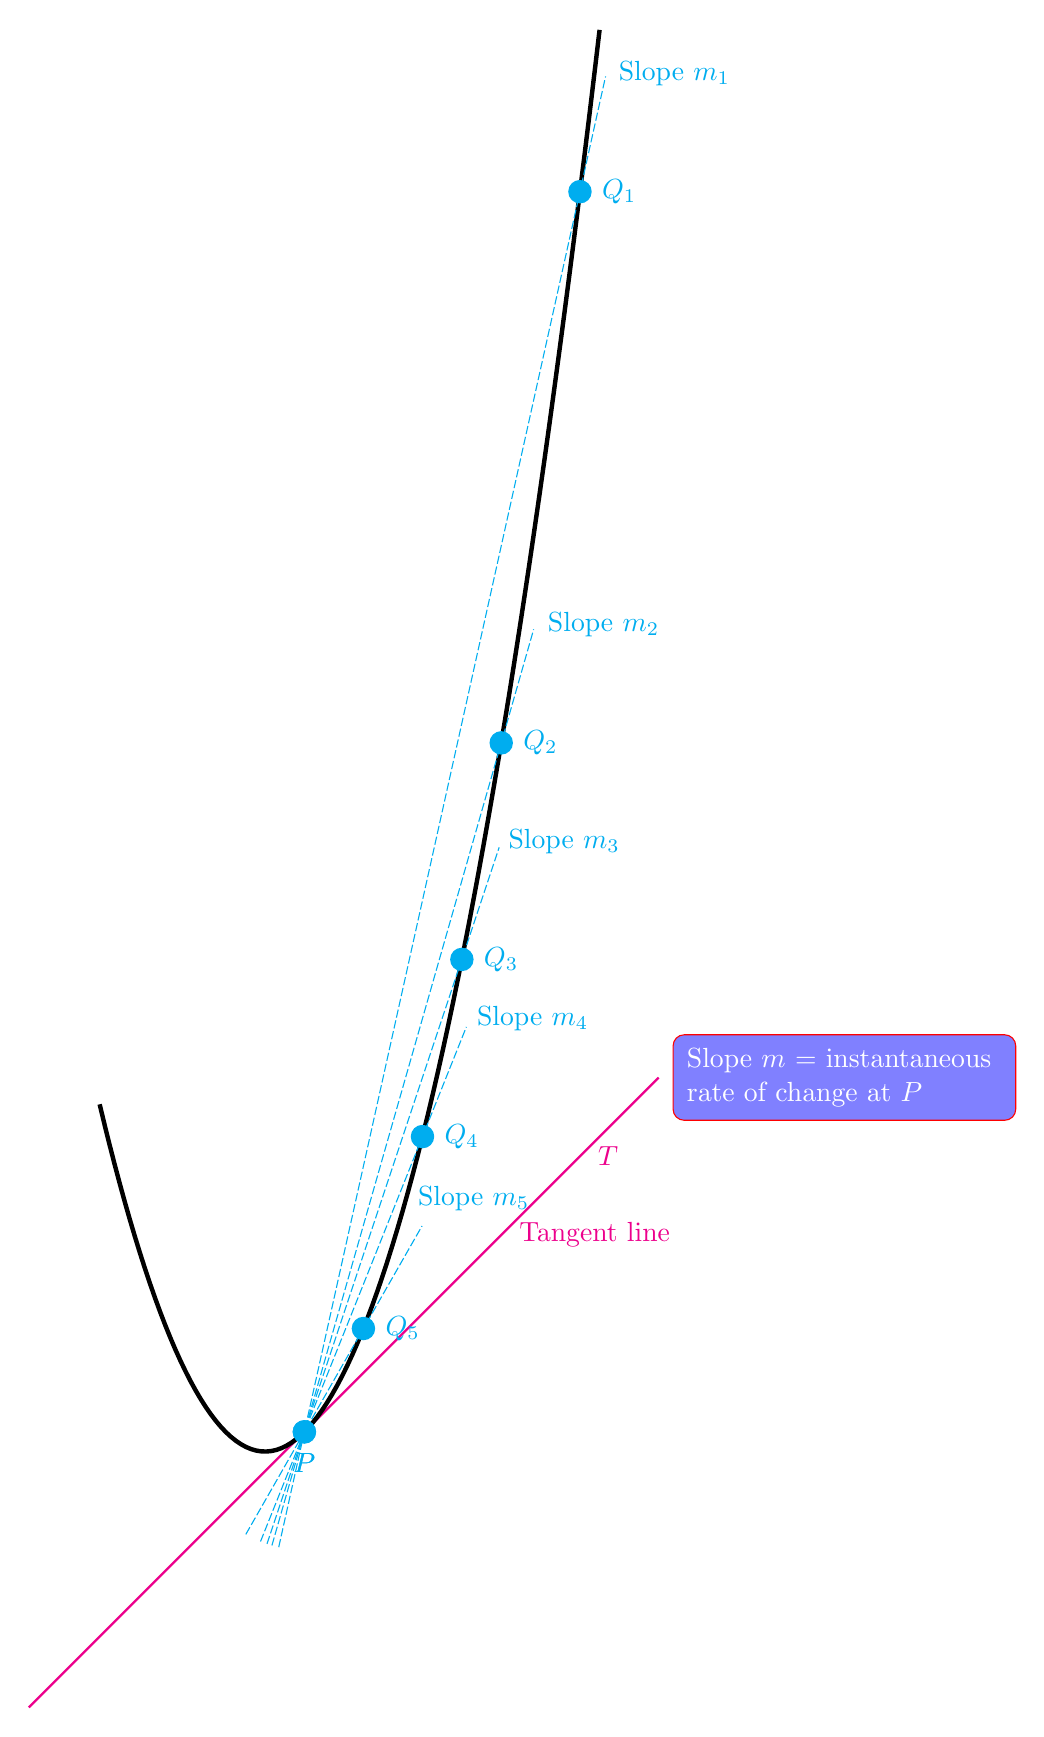
\begin{tikzpicture}
        \coordinate (P) at (2.5, 0.25);
        \coordinate (Q5) at (3.25, 1.5625);
        \coordinate (Q4) at (4, 4);
        \coordinate (Q3) at (4.5, 6.25);
        \coordinate (Q2) at (5, 9);
        \coordinate (Q1) at (6, 16);
        
        \draw[thick, magenta] plot[smooth, domain=-1:7] (\x, {\x - 2.25});
        \draw[ultra thick] plot[samples=100, domain=-0.1:6.25] (\x, {\x*\x - 4*\x + 4});
        
        \draw[cyan, dashed line] (P) node[dot, label={below:$P$}] {} -- (Q5) node[dot, label={right:$Q_5$}] {} node[shift={(1.4cm, 1.65cm)}] {Slope $m_5$};
        \draw[cyan, dashed line] (P) node[dot, label={below:$P$}] {} -- (Q4) node[dot, label={right:$Q_4$}] {} node[shift={(1.4cm, 1.5cm)}] {Slope $m_4$};
        \draw[cyan, dashed line] (P) -- (Q3) node[dot, label={right:$Q_3$}] {} node[shift={(1.3cm, 1.5cm)}] {Slope $m_3$};
        \draw[cyan, dashed line] (P) -- (Q2) node[dot, label={right:$Q_2$}] {} node[shift={(1.3cm, 1.5cm)}] {Slope $m_2$};
        \draw[cyan, dashed line] (P) -- (Q1) node[dot, label={right:$Q_1$}] {} node[shift={(1.2cm, 1.5cm)}] {Slope $m_1$};
        
        \draw (5, 2.75) node[right=3pt, magenta] {Tangent line};
        \draw (6, 3.75) node[right=3pt, magenta] {$T$};
        \draw (7, 4.75) node[right=5pt, text width=4cm, fill=blue!50, text=white, rounded corners, inner sep=5pt, draw=red] {Slope $m$ = instantaneous rate of change at $P$};
    \end{tikzpicture}
\end{document}